\documentclass[11pt,a4paper]{article}
\usepackage[a4paper,left=1in, right=1in, top=1.5in, bottom=1.2in]{geometry}
\usepackage[latin1]{inputenc}
\usepackage{amsmath}
\usepackage{amsfonts}
\usepackage{amssymb}
\usepackage{graphicx}
\usepackage{cite}
\usepackage{enumitem}
%\usepackage{wasysym}
\usepackage[usenames,dvipsnames]{color}
\usepackage{tikz}
\usepackage{gantt}
\usepackage{caption}
\usepackage{enumitem}
\usepackage{comment}
\usepackage{textcomp}
%\excludecomment{thebibliography}


\usepackage{fancyhdr}
\setlength{\headheight}{0.4in}
\pagestyle{fancy}
\lhead{\textsc{{\large Transitions to Renewable Energy: \\
Modeling it from the Bottom-up and the Top-down
 }}}
\chead{}
\rhead{}

\lfoot{\textsc{Project Description}}
\cfoot{\textsc{Haney, Carbajales-Dale, Heun}}
\rfoot{\thepage}

\renewcommand{\headrulewidth}{0.4pt}
\renewcommand{\footrulewidth}{0.4pt}



\begin{document}


%\maketitle



%\maketitle

%\begin{itemize}
%	\item 	clear statement of the work to be undertaken 
%	\item 	objectives for the period of the proposed work and expected significance 
%	\item 	relation to longer-term goals of the PI's project 
%	\item	relation to the present state of knowledge in the field, 
%	\item	relation to work in progress by the PI under other support and to work in progress elsewhere
%	\item	outline the general plan of work, including:
%	\begin{itemize}
%		\item	broad design of activities to be undertaken,
%		\item	clear description of experimental methods and procedures. 
%	\end{itemize}
%	\item Proposers should address 
%	\begin{itemize}
%		\item	what they want to do, 
%		\item	why they want to do it, 
%		\item	how they plan to do it, 
%		\item	how they will know if they succeed, and 
%		\item	what benefits could accrue if the project is successful. 
%	\end{itemize}
%	\item	must contain, as a separate section within the narrative, a discussion of the broader impacts of the proposed activities.
%\end{itemize}	
%
%\part{What we want to do}

%Page 1, First sentence --- “The objective of this proposal is to…..”
%Page 1, first paragraph: Overview of the project concisely identifying knowledge gaps (page 5 below) and how great you/your team is with the clever ways you will solve the knowledge gaps (page 6-7 below) 
%Page 1-3: Background information giving the state of the art in your science/engineering field. Be sure to include your own contributions. 
%Page 4-5: knowledge gaps: Identify what is wrong with the state of the art. Explain what you will cover in this proposal and what you won’t cover (and why). 
%Page 5-7: Clearly and concisely discuss how you are going to address the knowledge gaps with a series of specific hypotheses and objectives. A table linking hypotheses, objectives, and tasks is quite effective (Write this section first)
%Page 7-13: Detailed task descriptions. Show how tasks are interrelated. 
%Page 14: Listing of personnel and qualifications to show reviewers that you can do the work proposed above
%Page 15: Impact, what “product” will you deliver to the funding agency. 

\begin{table}
\begin{tabular}{lp{12cm}}
	\textsc{PI} & \textsc{Dr. Becky Haney, Economics, Calvin College, Grand Rapids, MI 49546}	\\
	\textsc{co-PI} & \textsc{Dr. Michael Carbajales-Dale, Environmental Engineering \& Earth Sciences, Clemson University, Clemson SC 29634} \\
	\textsc{co-PI} & \textsc{Dr. Matthew Heun, Engineering, Calvin College, Grand Rapids, MI 49546} \\
\end{tabular}
\end{table}
\section{Brief Description}
The objective of this prposal is to examine the economy as a complex 
adaptive system undergoing the process of transition from nonrenewable to renewable
energy resources while coupled with the natural system . As a complex adaptive system, the economy can exhibit
path-dependence and discrete jumps in technology rather than smooth transitions.
Because of the pervasiveness of energy consumption across
all sectors of the economy, the capital-intensive infrastructure that energy production and distribution
requires, and the time-lag between technological innovation in renewable
energy and implementation, the economy is at risk of sub-optimal
performance in the near-term transitions. At the same time,
dynamics within the natural system impact and are themselves impacted by
increasingly complex dynamics within the human-built system.


The schema in Figure~\ref{fig:CNH_Schema} describes the ways in which 
these human and natural systems processes are coupled.
\begin{figure}
\centering\
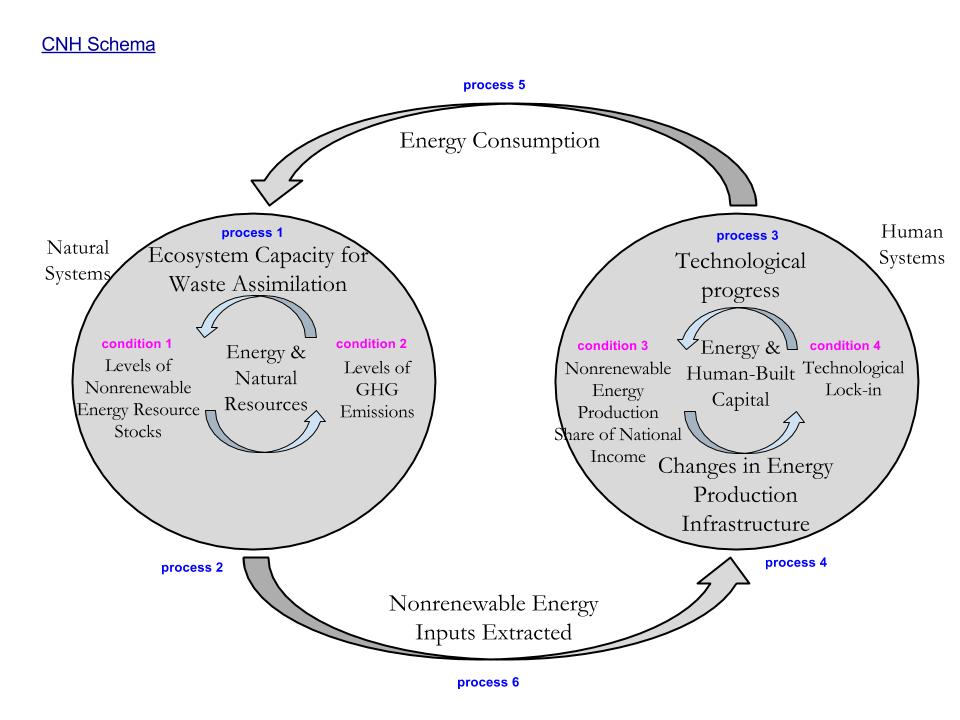
\includegraphics[width=\linewidth]{images/CNH_Schema.jpg}
\caption[CNH Schema]{CNH Schema for Energy Transitions.}
\label{fig:CNH_Schema}
\end{figure}
Over the course of the 21$^{st}$ Century, 
increasing social stressors, including
increased global population,
 higher living standards, and
improved access to modern energy infrastructure,
will place strong pressure on the capacity of the biosphere
to support such demands. 
In turn, biophysical stressors
such as climate change,
resource depletion, and
ecosystem degradation will make those demands
harder to meet.~\cite{IPCC2014}.
The modern industrial economy will be forced to undertake
transitions in the near future
to modes of operation that
(i) use renewable resources (such as forest products) 
at rates lower than their rate of regeneration;
(ii) emit wastes (such as carbon dioxide) 
at rates lower than their assimilation by environmental systems; and
(iii) reduce the use of non-renewable resources (such as crude oil) 
to rates at which renewable substitutes can be deployed~\cite{Goodland1996, G-R1971}. 

Those transitions are going to happen. What is not known, is how
those transitions will take place. In the words of the Shell Energy Scenarios, will there be an organized "blueprint"
for the transition, or a chaotic "scramble?"~\cite{} Mainstream economic models and the corresponding
policy planning cast (`top-down') infrastructure investment decisions 
within the economy as undertaken via a central agency,
with perfect knowledge and perfect foresight, 
or with some randomly generated, 
exogenously defined level of `uncertainty'~\cite{Hu2010}.
The structure of such models
is implicitly founded upon the existence both 
an equilibrium state for the economy
and an optimal pathway to reach that state~\cite{}.

In rejection to this perspective,
researchers in non-equilibrium and complexity economics
seek to understand the economy as a 
thermodynamically open system in a state of dynamic balance
with both the social and natural systems within which it is embedded~\cite{}.
From such a perspective the notion of `optimality' is lost,
instead economic interactions must instead be understood
`bottom-up' via the transaction and investment decisions
undertaken by multitudinous actors seeking to 
satisfice among multiple competing needs and wants~\cite{}.

Within this new framework,
agent-based modeling has become an important tool.
This project will an agent-based model to capture the 
complex dynamics of infrastructure development 
and change during the transition in energy sources. 

Creating a more resilient future
relies on decision making informed by 
economic, 
social,
and physical factors~\cite{Heun2015}.
The new era of resource depletion requires
new models of our economies that bridge the financial and physical
and that account for their inherent complexity.
Such models can guide advantageous (as opposed to optimal)
asset investment and resource consumption strategies
that are responsive to the constantly evolving 
social and environmental landscape.

The proposed project will build on an agent-based model
developed by the project PI to answer the following questions:
\begin{enumerate}
\vspace{-9pt}
\setlength{\itemsep}{-3pt}
	\item	are multiple, interacting agents able to collectively manage 
				a transition from non-renewable to renewable resources 
				to avoid negative impacts of resource depletion?
	\item	if yes, do there exist resource consumption and investment decisions
				that are more advantageous in managing this transition?
\end{enumerate}


%\section{Problem statement}
%\label{sec:problem}
%
%\subsection{Significance of the problem}

In order to answer these questions,
this research will explore the behavior of agents in 
a resource harvesting and investment simulation where 
resource managers must forage for energy and natural resources 
while investing some of those resources towards the activities of foraging 
while also maintaining and building out critical infrastructure. 
In autonomous mode (agents act according to built-in algorithms), 
advantageous strategies for resource management can be 
`evolved' through the process of `natural selection'. 
In learning mode (researchers or learners take control of the agent behavior), 
successive rounds of the simulation will more closely resemble real-world locations. 
Researchers can better understand the context for 
resource and infrastructure management strategies 
with the aim of developing more informed policies.

Comparison of simulation results of agent-based models to real-world otucomes 
is key to assessing their validity. Matthew Heun, 
a Co-PI on the project, will be building a unique data on the South African energy infrastructure 
that will be a plumb line to compare and contrast the "top-down" and "bottom-up" models of the economy.




\newpage



\bibliography{ABM}
\bibliographystyle{unsrt}



\end{document}